\section{New RIMs in a Dynamic PRA Context}
\label{sec:newRIM}

Note that the RIMs described so far are tight to a binary logic of the outcome 
variable (e.g., OK vs. CD). Dynamic PRA approaches typically generate a continuous 
value of the outcome variables (e.g., peak clad temperature - $PCT$). 
In our application (see previous sections) we typically convert $PCT$ to a discrete 
one as follows:
\begin{itemize}
  \item $PCT>2200 F$: outcome = CD
  \item $PCT<2200 F$: outcome = OK
\end{itemize}
  
Given the different structure of the approach used in this paper to solve a PRA 
problem (i.e., Dynamic instead of classical PRA), the reader might think that a different 
set of RIMs should/could be developed in order to capture the nature of the problem 
solved using Dynamic PRA.
As a starting point, it would worth investigating the nominal probabilistic distribution 
(pdf) of PCT with the one obtained when reliability of each basic event (sampled parameter) 
is 0.0 or 1.0. So now we can indicate:
\begin{itemize}
  \item $pdf_0 (T)$: nominal pdf of PCT
  \item $pdf_i^-(T)$: pdf of PCT associated to basic event $i$ assuming basic event is perfectly 
        reliable
  \item $pdf_i^+(T)$: pdf of PCT associated to basic event $i$ assuming basic event has failed
\end{itemize}

An example is shown below for a hypothetical case where obtained $pdf_0(T)$ is indicated 
using an histogram while the limit value for PCT is shown using the red line passing at 2200 F.
In order to make a connection to what has been presented in the previous section, note that by 
looking at Fig.~\ref{fig:margin0}:
\begin{equation}
  R_0 = \int_{2200}^\infty \! pdf_0(T) \, dT
  \label{eq:R0}
\end{equation}

As part of the RISMC analysis, the user might want to supplement the results obtained in the 
previous section with the information associated to a more effective margin analysis.
In particular, of interest for RISMC applications is (see Fig.~\ref{fig:margin0}) the concept of margin:
\begin{equation}
  margin= 2200-PCT \text{ given } PCT<2200
  \label{eq:margin}
\end{equation}

\begin{figure}
  \centering
  \begin{subfigure}{.5\textwidth}
    \centering
    \centerline{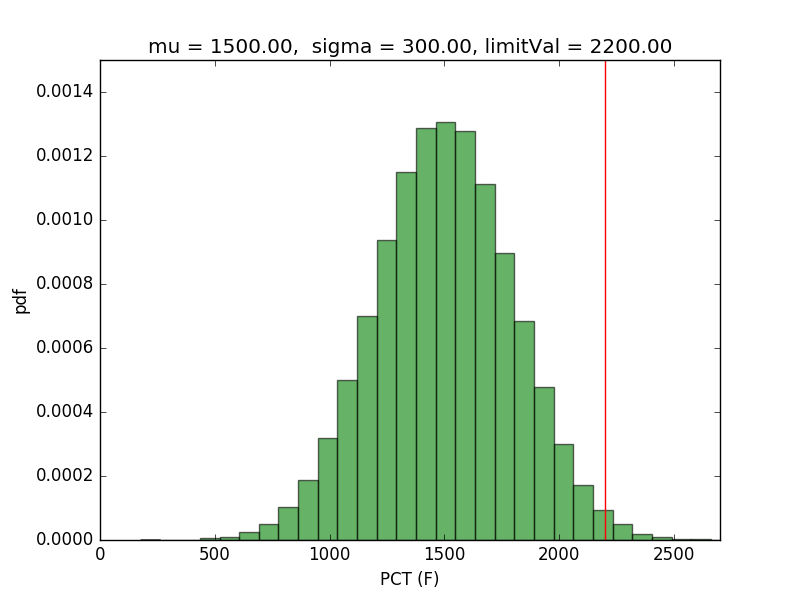
\includegraphics[scale=0.3]{pdf0.png}}
  \end{subfigure}%
  \begin{subfigure}{.5\textwidth}
    \centering
    \centerline{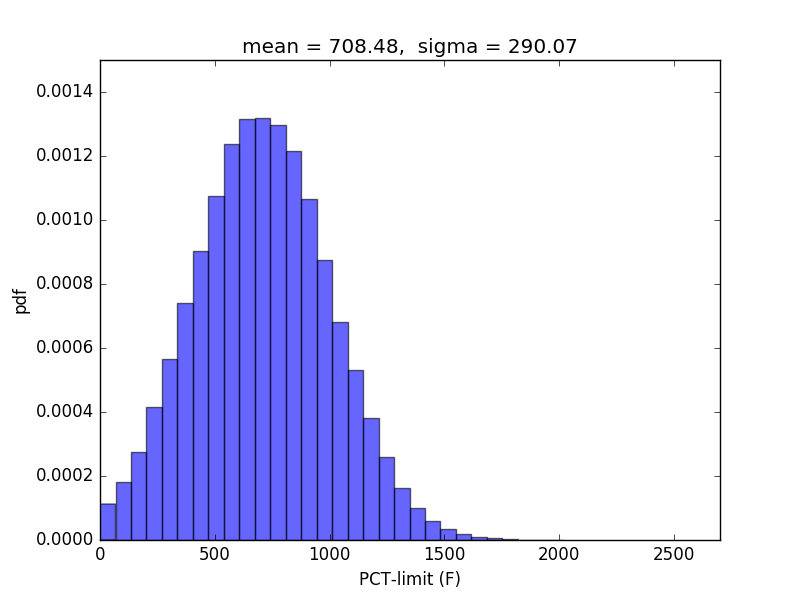
\includegraphics[scale=0.3]{margin0.png}}
  \end{subfigure}
  \caption{Plot of a hypothetical $pdf_0(T)$ (left) and its associated margin $margin_0$ (right).}
  \label{fig:margin0}
\end{figure}
 
Using the same philosophy indicated in the previous section for classical RIMs, we want 
to determine:
\begin{itemize}
  \item $margin_0$: pdf of the variable $2200-PCT$ given that $PCT<2200$
  \item $margin_i^-$: pdf of the variable $2200-PCT$ given that $PCT<2200$ for basic 
                      event $i$ assuming it is perfectly reliable
  \item $margin_i^+$: pdf of the variable $2200-PCT$ given that $PCT<2200$ for basic event 
                      $i$ when its assumed to be failed
\end{itemize}

Note now that $margin_0$, $margin_i^-$ and $margin_i^+$ are now pdfs and not numerical values. 
Hence, now the challenge arises on how to compare two pdfs:
\begin{itemize}
  \item $margin_0$ vs. $margin_i^-$
  \item $margin_0$ vs. $margin_i^+$
\end{itemize}

\begin{figure}
  \begin{subfigure}{.5\linewidth}
  \centering
  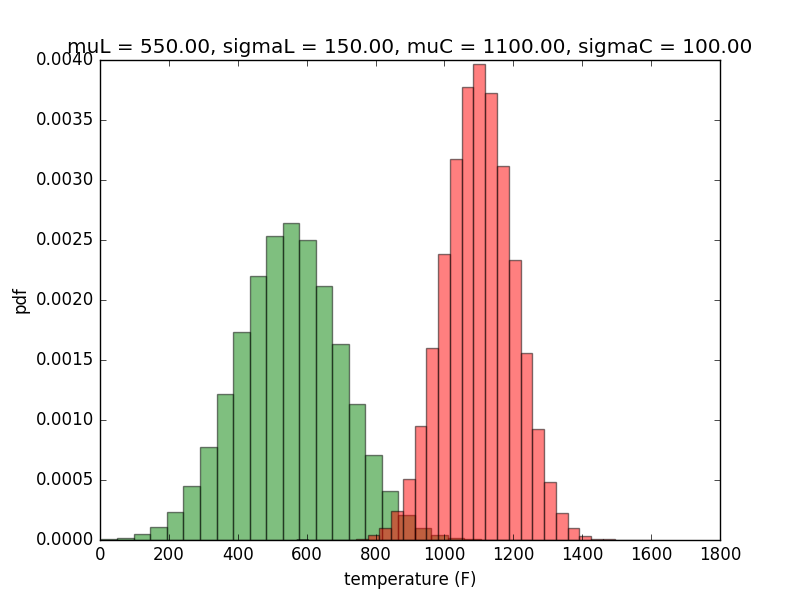
\includegraphics[scale=.3]{dist_dist_1.png}
  \end{subfigure}%
  \begin{subfigure}{.5\linewidth}
  \centering
  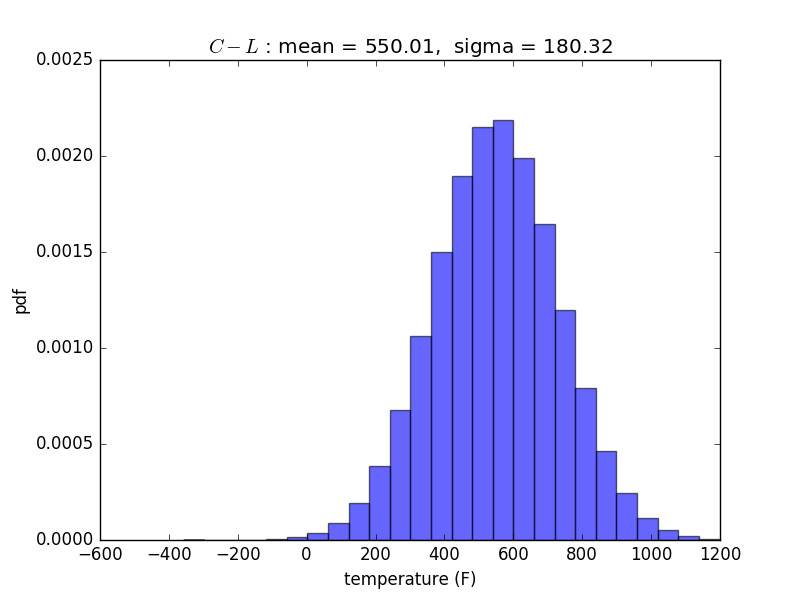
\includegraphics[scale=.3]{dist_dist_2.png}
  \end{subfigure}\\[1ex]
  \begin{subfigure}{\linewidth}
  \centering
  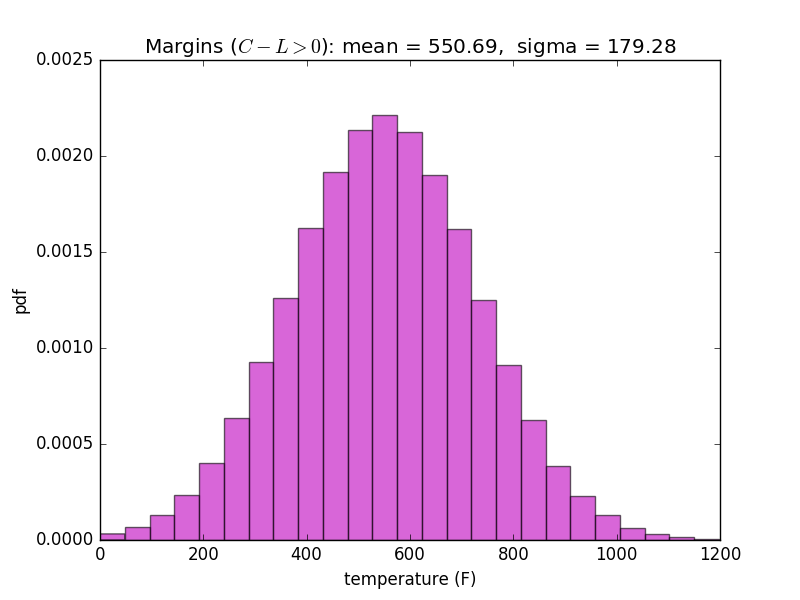
\includegraphics[scale=.3]{dist_dist_3.png}
  \end{subfigure}
  \caption{Plot of the pdfs for $PCT$ (green) and $CFT$ (red) (top left), 
           Plot of the pdf of the variable $CFT-PCT$ (top right) and 
           Plot of the pdf of the margin, i.e., $CFT-PCT>0$ (bottom).}
  \label{fig:dist_dist}
\end{figure}

Assume two pdfs are given: $pdf_1(x)$ and $pdf_2(x)$. Few approaches can be followed: Z-test or 
Kolmogorov–Smirnov test. 
In the first approach (Z-test), the following variable $Z$ is computed:
\begin{equation}
  Z_{1,2} = \frac{mean(pdf_1)-mean(pdf_2)}{\sqrt{std\_dev^2 (pdf_1)-std\_dev^2(pdf_2)}} 
  \label{eq:Ztest}
\end{equation}
where:
\begin{itemize}
  \item $mean(pdf)$ correspond to the mean of $pdf(x)$ 
  \item $std\_dev(pdf)$ correspond to the standard deviation of $pdf(x)$ 
\end{itemize}

In the second approach (Kolmogorov–Smirnov test~\cite{}), instead of the pdf, the cumulative 
distribution functions (pdf) are considered: $cdf_1(x)$ and $cdf_2(x)$. 
In particular, the Kolmogorov-Smirnov statistic is calculated as:
\begin{equation}
  Z_{1,2} = \sup_{x} (cdf_1(x) - cdf_2(x))
  \label{eq:Kolmogorov-Smirnov}
\end{equation}

Note that so far we have imposed clad failure temperature ($CFT$) to be a fixed value, 
i.e., 2200 F. 
In many RISMC applications $CFT$ is no longer a numerical value but it can be un uncertain 
parameter, i.e., a pdf is associated to CDF: $pdf(T)$. 
This link goes back to the original logo of RISMC where a pdf for ``load'' and ``capacity'' 
(see Fig.~\ref{}).
A new definition of margin can be then defined:

\begin{equation}
  margin=(CFT-PCT) \text{ given } (CFT-PCT>0)
  \label{eq:new margin}
\end{equation}

From here, once the pdf associated to the margin variable is determined it is possible 
to employ either the Z-tests or the Kolmogorov–Smirnov test in order to measure how this pdf 
changes when each basic event is considered perfectly reliable or failed. 
